\documentclass[12pt]{letter}
\usepackage[utf8]{inputenc}
\usepackage{graphicx}
\usepackage{eurosym}
\usepackage{charter}
\usepackage{hyperref}  
\usepackage{xcolor}  

\hypersetup{
    colorlinks,
    linkcolor=[HTML]{404040},
    urlcolor={blue!50!black}
}

\signature{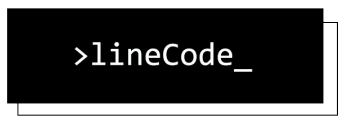
\includegraphics[scale=0.5]{../../commons/res/lclong.png} \\
			Giacomo Bulbarelli  \\ 
			\textit{Responsabile di progetto}
			\href{}{}}
\address{ Via Trieste, 63 \\ Padova \\ 35121 PD, Italia}

\date{10 gennaio 2021}

\begin{document}

\begin{letter}{ }

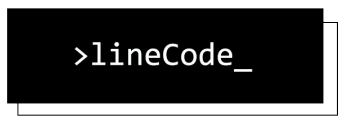
\includegraphics[scale=0.5]{../../commons/res/lclong.png}

\opening{Gentile prof. Vardanega,\\ Gentile prof. Cardin, }

Con la presente il gruppo 9, \textit{lineCode}, vuole confermare la volontà di realizzazione del prodotto dal titolo 
\textbf{PORTACS (Capitolato 5)}, da Voi commissionato e proposto dall'azienda \textit{Sanmarco Informatica}. \\
Inoltre, comunichiamo che i costi preventivati per lo sviluppo del prodotto sono pari a \EUR{}13.124,00.


Le forniamo il link di una repository pubblica da cui è possibile scaricare e visualizzare online i documenti richiesti dal progetto.
In particolare:

\begin{itemize}
	\item \textit{Analisi dei Requisiti v1.0.0};
	\item \textit{Piano di Qualifica v1.0.0};
	\item \textit{Piano di Progetto v1.0.0};
	\item \textit{Norme di Progetto v1.0.0};
	\item \textit{Studio di Fattibilità v1.0.0};
	\item \textit{Glossario v1.0.0};
	\item \textit{verbali interni};
	\item \textit{verbali esterni}.
\end{itemize}

\newpage

Vengono anche riportati i nominativi e numeri di matricola dei membri del gruppo. Nello specifico:

\begin{center}
   \centering
   \begin{tabular}{ll}
     \textbf{Nominativo}        & \textbf{Matricola} \\
     Matteo Alba                     &  1075682 \\
	 Giacomo Bulbarelli              &  1144046 \\
	 Alessandro Chimetto             &  1142192 \\     
	 Alessandro Dindinelli           &  1170457 \\	     
	 Lucia Fenu                      &  1125521 \\
     Paolo Scanferlato               &  1170709 \\
     Valton Tahiraj                  &  1193389 \\
   \end{tabular}
 \end{center}

Il link per scaricare e visualizzare i documenti è il seguente:

\begin{center}
\href{https://drive.google.com/drive/folders/1N6tddrSkpzLvGaf5xY4jaPSYzu2QkPc7?usp=sharing}{Cartella condivisa su Google Drive}
\end{center}

Nel caso in cui il link nel documento non dovesse funzionare, il riferimento esplicito è il seguente:
\begin{center}
https://drive.google.com/drive/folders/1N6tddrSkpzLvGaf5xY4jaPSYzu2QkPc7?usp=sharing
\end{center}


Per qualunque altro chiarimento o problema, rimaniamo a completa disposizione.

\closing{Cordiali saluti,}


\vspace{3em}

\end{letter}

\end{document}
